\section{Probabilistic Planning}
\subsection{Markov Decision Processes}
An MDP is specified by a quintuple: $(X, A, r, P(x'|x, a), \gamma)$, where $X$ are states, $A$ are actions, $r(x,a)$ is a reward function and transition probabilities:\\
    $P(x'|x,a)=\text{Prob(Next state}=x'|\text{Action } a)$\\ 
\textbf{Objective:} find a stationary policy $\pi: S \rightarrow A$ that maximizes the sum of cumulative rewards.
\textbf{Value of a state given a policy :} sum of cumulative rewards, given that the initial state is this state $\rightarrow$ \textbf{Bellman equation:}\\
$V^\pi(s)=\mathbb{E}\Big[ \sum_{t=0}^\infty \gamma^tr(s_t, \pi(s_t), s_{t+1})|s_0=s\Big]$\\
$= \sum_{s'\in S}P(s'|s, \pi(s))\big[r(s, \pi(s),s')+\gamma V^\pi(s')\big]$\\
$= r(s, \pi(s))+\gamma\sum_{s'\in S}P(s'|s,\pi(s))V^\pi(s')$

% 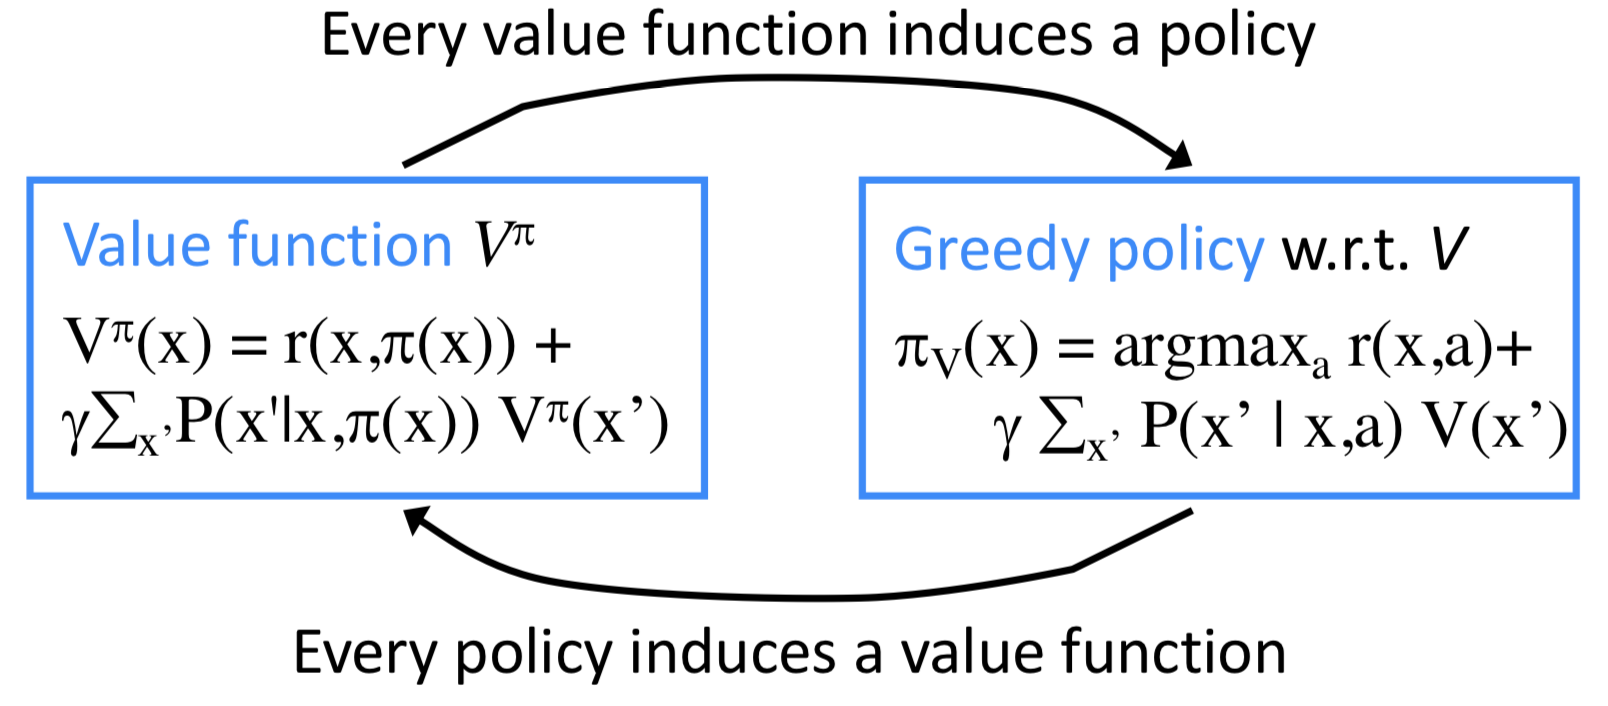
\includegraphics[scale=0.25]{valueFunctionAndPolicy.png}
\textbf{Theorem (Bellman)}: a policy is optimal iff it is greedy w.r.t. its induced value function!\\
$V^*(x)=max_a[r(x,a)+\gamma \sum_{x'}P(x'|x,a)V^*(x')]$\\
Bellman equation mais geral: \\
$V^*(x)=max_a[ \sum_{x'}P(x'|x,a)(r(a, x, x')+\gamma V^*(x')])$
Optimal policy: \\
$\pi^*(s)=\underset{a\in A}{argmax} [r(x,a)+\gamma \sum_{x'}P(x'|x,a)V^*(x')]$

\subsection{Policy iteration (Cost $O(S^3+SA\Delta)$)}
Start with an arbitrary (e.g. random) policy $\pi$.
Until converged, do:\\
- Compute value function $V^\pi (x)$\\
- Compute greedy policy $\pi_G$ w.r.t. $V^\pi$\\
- Set $\pi \leftarrow \pi_G$\\
Guaranteed to monotonically improve and to converge to an \textbf{optimal} policy $\pi^*$ in $O(n^2m/(1-\gamma))$ iterations (converges in polynomial number of iterations)!

\subsection{Value iteration (Cost $O(SA\Delta)$)}
Initialize $V_0(x)=max_a r(x,a)$\\
For $t=1$ to $\infty$:\\
- For each $(x,a)$, let: \\
$Q_t(x,a)=r(x,a)+\gamma\sum_{x'}P(x'|x,a)V_{t-1}(x')$\\
- For each $x$, let $V_t(x)=\underset{a}{max}Q_t(x,a)$\\
- Break if $||V_t-V_{t-1}||_{\infty}=\underset{x}{max}|V_t(x)-V_{t-1}(x)|\leq\epsilon$\\
Then choose greedy policy w.r.t $V_t$.\\
Guaranteed to converge to $\epsilon$-optimal policy (finds approximate solution in polynomial number of iterations)!

\subsection{POMDP = Belief-state MDP}
States = beliefs over states for original POMDP\\
$B=\Delta({1,...,n})=\{ b:{1,...,n} \rightarrow [0,1],\sum_x b(x)=1 \}$\\
Actions: same as original MDP\\
\textbf{Transition model:}\\
- Stochastic observation:\\
$P(Y_t|b_t)=\sum_{x=1}^n P(Y_t|X_t=x)b_t(x)$\\
- State update (Bayesian filtering!), given $b_t, y_t, a_t$:
$b_{t+1}(x')=\frac{1}{Z}\sum_xb_t(x)P(y_t|x)P(X_{t+1}=x'|X_t=x,a_t)$\\
Reward function: $r(b_t, a_t)=\sum_x b_t(x)r(x,a_t)$

\subsection{Example of approx. solution to POMDPs: Policy gradients}
- Assume parameterized policy: $\pi(b)=\pi(b;\theta)$\\
- For each parameter $\theta$ the policy induces a Markov chain\\
- Can compute expected reward $J(\theta)$ by sampling.\\
- Find optimal parameters through search (gradient ascent):
$\theta^* = \underset{\theta}{arg max}\quad J(\theta)$


